\documentclass[12pt,a4paper,titlepage,twoside]{book}
\usepackage[margin=0.75in,footskip=0.25in]{geometry}
\usepackage[latin1]{inputenc}
\usepackage{amsmath}
\usepackage{fancyhdr}
\usepackage{multirow,tabularx}
\usepackage{amsfonts}
\usepackage{amssymb}
\usepackage{makeidx}
\usepackage{graphicx}
\usepackage{pgfgantt}
\usepackage{multirow}
\usepackage{array}
\usepackage{tabularx}
\usepackage{longtable}
\usepackage{pdfpages}
\usepackage{fullpage}
\title{ IoT enabled smart switchboard to enable remote control of existing home appliances }
\author{Capstone Project}
\begin{document}
    \begin{titlepage} 
    	\newcommand{\HRule}{\rule{\linewidth}{0.4mm}}
    	\centering 
    	\textsc{\Large UEE693}\\[0.5cm] 
    	\textsc{\large Capstone Project}\\[0.5cm]
    	\HRule\\[0.4cm]
    	{\huge\bfseries IoT enabled smart switchboard to enable remote control of existing home appliances}\\[0.4cm]
    	\HRule\\[1.5cm]
    	\vfill
    	\begin{minipage}{0.5\textwidth}
    		\begin{flushleft}
    			\large
    			\textit{Investigating Group}\\[0.25cm]
    			101504114 Satyam Kumar\\
    			101504119 Shubham Gupta\\
    			101504120 Stuti Sidhu\\
    			101504122 Swanav\\
    		\end{flushleft}
    	\end{minipage}
    	~
    	\begin{minipage}{0.4\textwidth}
    		\begin{flushright}
    			\large
    			\textit{Supervisor}\\
    			Dr. Mukesh Singh
    		\end{flushright}
    	\end{minipage}
    	\vfill\vfill\vfill
    	{\large 2018-19}		
    	\vfill\vfill
    	\includegraphics[width=0.3\textwidth]{logo.png}\\
    	Electrical and Instrumentation Engineering Department\\
    \end{titlepage}
    
    \tableofcontents
    \newpage
    \frontmatter
	    \chapter*{Declaration}
    \addcontentsline{toc}{section}{Declaration}
    
    We hereby declare that the project entitled \textbf{"IoT enabled smart switchboard to enable remote control of existing home appliances"} is an authentic record of our own work carried out in the \textit{Electrical \& Instrumentation Engineering Department, Thapar University, Patiala} under the guidance of \textit{Dr. Mukesh Singh} during 6th and 7th semester (2018).\\\\
    \hspace*{\fill} \textbf{Date: }\today \\
	\vfill
	\vfill
	\begin{minipage}{0.5\textwidth}
		\begin{flushleft}
			\large
				\begin{tabular}{l l}
					\multicolumn{2}{c}{\textit{Investigating Group}} \\
					Satyam Kumar   & 101504114 \\
					Shubham Gupta  & 101504119 \\
					Stuti Sidhu    & 101504120 \\
					Swanav Swaroop & 101504122 \\
				\end{tabular}
			
		\end{flushleft}
	\end{minipage}
	~
	\begin{minipage}{0.4\textwidth}
		\begin{flushright}
			\large
			\textit{Supervisor}\\
			Dr. Mukesh Singh
		\end{flushright}
	\end{minipage}
    \vfill
    
    
	    \chapter*{Acknowledgement}
    \addcontentsline{toc}{section}{Acknowledgement}
    We would like to extend our heartfelt gratitude to all those who have contributed towards the successful completion of the project and converge thanks to our supervisor \textit{Dr. Mukesh Singh} and all the faculty and staff at \textit{Electrical and Instrumentation Engineering Department (EIED)}, Thapar University for generously extending their support and for sparing their valuable time to guide us towards the completion of the project.
    We would like to thank all the group members whose responses and co-ordination were of utmost importance for the project.
    \vfill
    \vfill 
    \begin{center}
		\begin{tabular}{l l l l}
			Satyam Kumar&Shubham Gupta&Stuti Sidhu&Swanav Swaroop\\
			101504114&101504119&101504120&101504122\\
		\end{tabular}
    \end{center}
	\vfill
    
    
	    \chapter*{Abstract}
    \addcontentsline{toc}{section}{Abstract}
    
    A Smart Switch Board is a compact and efficient replacement of conventional switchboard, which provides the automated control to the user. It ensures the user convenience and energy saving via modern control strategy and power electronic devices. In addition, the unnecessary wastages of electricity can be prevented by controlling the appliances even from outside the house.\\
    
    The switches are made in modular fashion which provides the provision for scalability of the product as the user can increase the number of devices connected over time.  So it can be put forward for the commercialization purpose.\\
    
    The existing products available in the market requires replacement of the existing devices with the new smart devices which is quite costly and also the existing devices carry no use after that. The smart switch just upgrades the conventional switch boards and the existing devices then can be controlled over the internet.\\
    
    In this project we provide a 5V supply to the input of the microcontroller which provides gating signals to the driver circuit. A zero cross detection circuit is formed for calculating the time at which the rectified voltage reaches zero. Feeding these values in the microcontroller, it fires interrupts to flag the initiation of counter which provides delayed pulse according to the input provided by the user. Simulation and PCB design of the Circuit were made in Orcad Cadence Software.\\
    
    
	    \include{chapters/frontmatter/tables}
	    \include{chapters/frontmatter/figures}
	    \newpage
	    \chapter*{List of Abbreviations}
    \addcontentsline{toc}{section}{List of Abbreviations}
    
        
    \mainmatter
	    \chapter{Introduction}
        \section{Introduction}
        
        In the present day scenario, Energy efficiency is the major requirement of any power device (mechanical or electrical). By the introduction of Power Electronics systems electrical systems are aiming towards higher energy efficiency. The losses in these systems are quite low and they enable the user to control the devices to a much larger extent than was possible by using the conventional approach. \\
        
        This project focuses on providing automated control of the existing home appliances by adding a control circuitry to the existing devices. The devices are controlled using wireless communication over the internet by microcontrollers. An app-driven remote control is provided for user interaction. The efficiency of usage can be improved device-by-device. This will enable the user to switch off the devices when idle even remotely and also the power consumptions of devices will be lowered when appliances are not running at their full intensities. Cumulatively, an energy efficient household can be achieved by using such smart switches for controlling appliances used in the house. \\
        
        A smart switchboard is an upgrade to the conventional switches, they use novel Internet of Things (IoT) enabling them to be accessible remotely over the internet. The switches are designed in a modular fashion providing scope for scalability of the project. Based upon the monetary capability of the user and upon introduction of new devices in the household at later stages, the sockets can be easily added or removed at any time in the smart switch. This will enhance the viability and long term relevance of the project.\\ \newpage
        
        \section{Literature Survey}
        	\subsection{National Status Review}
        	\begin{itemize}
        		\item Archana N. Shewale, \textbf{"Renewable Energy Based Home Automation System Using ZigBee"}, International Journal of Computer Technology and Electronics Engineering (IJCTEE), 2015\\ \\
        		Archana N. Shewale describes the methodology of renewable energy based home automation in which two things are consider one is energy consumption and another is energy generation. In this, ZigBee is used for monitoring energy consumption of home equipment and power line communication (PLC) is used to monitoring energy generation.
        		\item S. Anusha, \textbf{"Home Automation using ATmega328 Microcontroller and Android application"}, International Research Journal of Engineering and Technology(IRJET), 2015\\ \\
        		S. Anusha describes the design and development of a remote household appliance control system using ATmega328 microcontroller and android mobile through GSM technology.
        		\item J. Chandramohan, \textbf{"Intelligent Smart Home Automation and Security System Using Arduino and Wi-Fi"}, International Journal of Engineering and Computer Science, 2017\\ \\
        		J. Chandramohan provides a low cost-effective and flexible home control and monitoring system with the aid of an integrated micro-web server with internet protocol (IP) connectivity for access and to control of equipment and devices remotely using Android-based smartphone application. generation.
        	\end{itemize}
        	\subsection{International Status Review}
        	\begin{itemize}
        		\item Debraj Basu, \textbf{"Wireless Sensor Network Based DSAda Smart Home: Sensor Selection, Deployment and Monitoring"}, IEEE, 2013\\ \\
        		Debraj Basu details the installation and configuration of unobtrusive sensors in an elderly person?s house - a smart home in the making - in a small city in New Zealand. The overall system is envisaged to use machine learning to analyze the data generated by the sensor nodes.
        		\item Byeongkwan Kang, \textbf{IoT-based monitoring system using tri-level context making model for smart home services"}, IEEE International Conference, 2015\\ \\
        		Kang discusses about acquisition and analysis of sensor data which are going to be used across smart homes. It proposed an architecture for extracting contextual information by analysing the data acquired from various sensors and provide context aware services.
        		\item Jeya Jeya Padmini, \textbf{"Effective Power Utilization and Conservation in Smart Home Using IoT"}, IEEE International Conference, 2015\\ \\
        		Jeya Jeya Padmini discusses about effective power utilization and conservation in smart homes using IoT. It uses cameras for recognizing human activities through image processing techniques.
        		\item Pranay P. Gaikwad, \textbf{"A Survey based on Smart Home System Using Internet of Things"}, IEEE International Conference, 2015\\ \\
        		Pranay P.Gaikwad discusses about challenges and problems arise in smart home systems using IoT and propose possible solutions.
        	\end{itemize}
        \section{Need Analysis}
        
        	The currently available solution and research exhibit these features
        	\begin{itemize}
        		\item The existing market solutions provide on/off switching of the devices. The available solutions provide comparatively lower energy efficiency and also require human intervention to achieve desired conditioning of the environment.
        		\item Some of them also use unsuitable technologies like Bluetooth, Ethernet etc. From the present analysis of the existing solutions for automating a room environment, the technologies used suffer from a number of drawbacks. So, these protocols are limited in functionalities when used by an end user in real life.
        	\end{itemize}
        	
        \section{Aim}
        	The project aims to manage and control existing devices through a smart switchboard accessible over the internet.
        	        \section{Objectives}
	        \begin{itemize}
	        	\item To develop driver circuits for controlling the devices inside a room
                 \item To develop software programs for the microcontroller to operate the driver circuits.
                  \item To design mobile applications for users to control the devices over the internet.
	        \end{itemize}
        \section{Problem Formulation}
        In the present day scenario, user comfort and convenience is the main target for the product developers. The present conventional devices installed and their manual control does not provide benefit for monitoring and controlling them, when a person is away from home. This leads to large power losses due to unnecessary operation of the devices. This can even cause major damages to life and property if not handled properly. Also, existing commercial solutions in the market provide entire new smart devices which requires users to replace the existing devices incurring huge costs. 
        \section{Deliverables}
        	\begin{itemize}
        		\item A compact and efficient Smart Switch Board is developed.

                 \item A user-friendly mobile application is developed for operating different appliances installed inside the room.
        	\end{itemize}
        \section{Novelty of work}
        Devices can be controlled over the internet through mobile or desktop applications. Due to the use of Power Electronics devices for the voltage control, there are negligible losses incurred. The switches are formed in a modular fashion providing user to add new devices over time. Higher levels of controllability could be achieved through individual device level control.	
    
	    \chapter{Theory, Standards and Constraints}
        \section{Theory}
        
        The schematic consists of three main components working in conjugation to provide internet of things enabled device control.
        
        \subsection{5V Power Supply}
        	A 5V Power supply is designed to provide uninterrupted mains supply to the microcontroller.\\
        	The 230V AC Mains is converted to a 13V AC signal using a Step Down Transformer. The transformer also provides isolation to the circuit. This stepped down voltage is passed through a bridge rectifier to convert it into a pulsating DC output. This DC supply cannot be reliably without converting removing ripples from the output and thereafter regulating the output. Hence, this output is connected to a LM7805 5V Voltage Regulator in parallel with 2200 \si\micro f and a 470 \si\micro f capacitors. This stabilises the output and reduces the input ripples to almost zero.
        	
        	\begin{figure}[h!]
        		\includegraphics[width=\textwidth]{photos/ckt-dgm/5VDCPowerSupply.jpg}
        		\caption{5V DC Power Supply}
        	\end{figure}
        	
        \subsection{Phase Angle Control}
        	Phase angle control is a simple AC-AC conversion technique used to convert an input AC RMS Voltage to a reduced RMS value.\\
        	It uses a low frequency switch to chop the AC sine wave. The reduced output voltage is controlled using a quantity known as the \textbf{Firing Angle}. The firing angle determines when the Sine Wave is chopped.\\
        	The output voltage is calculated by the determinig the area under the curve, hence the integral of a sine wave from the firing angle to the zero crossing angle.\\
        	There are a variety of benefits of this approach:
        	\begin{itemize}
        		\item This allows the use of a low frequency switch, in our case a Triac.
        		\item A Triac can sustain higher power output
        	\end{itemize}
        	
        
    \subsection{ESP8266}
        \begin{wrapfigure}{r}{0.3\textwidth}
        	\includegraphics[width=0.3\textwidth]{photos/theory/esp8266.jpg}
        	\caption{ESP8266 Wifi Microcontroller}
        \end{wrapfigure}
    
        The ESP8266 WiFi Module has a self contained SOC with an integration of TCP/IP protocol stack which can provide any microcontroller access to the Wifi network. The ESP8266 has the potential of either hosting an application or offloading all Wi-Fi networking functions from another application processor. Each ESP8266 module comes pre-programmed with an AT command set firmware, meaning, you can simply hook this up to your Arduino device and get about as much WiFi-ability as a WiFi Shield offers (and that just out of the box). The ESP8266 module is an extremely cost effective board with a huge, and ever growing, community.\\
        
        This module has a powerful enough on-board processing and storage capability that allows it to be integrated with the sensors and other application specific devices through its GPIOs with minimal development up-front and minimal loading during runtime. Its high degree of on-chip integration allows for minimal external circuitry, including the front-end module, is designed to occupy minimal PCB area. The ESP8266 supports APSD for VoIP applications and Bluetooth co-existance interfaces, it contains a self-calibrated RF allowing it to work under all operating conditions, and requires no external RF parts.
\subsection{Triac}
The TRIAC is an ideal device to use for AC switching applications because it can control the current flow over both halves of an alternating cycle. A thyristor is only able to control them over one half of a cycle. During the remaining half no conduction occurs and accordingly only half the waveform can be utilised.\\

\begin{wrapfigure}{r}{0.3\textwidth}
	\includegraphics[width=0.3\textwidth]{photos/theory/bt136.jpg}
	\caption{Triac BT136}
\end{wrapfigure}
Seen from the outside it may be viewed as two back to back thyristors and this is what the circuit symbol indicates.On the TRIAC symbol there are three terminals. These are the Gate and two other terminals are often referred to as an "Anode" or "Main Terminal". As the TRIAC has two of these they are labelled either Anode 1 and Anode 2 or Main Terminal, MT1 and MT2.
The TRIAC is a component that is effectively based on the thyristor. It provides AC switching for electrical systems. Like the thyristor, the TRIACs are used in many electrical switching applications. They find particular use for circuits in light dimmers, etc., where they enable both halves of the AC cycle to be used. This makes them more efficient in terms of the usage of the power available. While it is possible to use two thyristors back to back, this is not always cost effective for low cost and relatively low power applications.

\subsection{MOC3021 and MOC3041 Optocouplers}
An opto-isolator (also called an optocoupler, photocoupler, or optical isolator) is an electronic component that transfers electrical signalsbetween two isolated circuits by using light. Opto-isolators prevent high voltages from affecting the system receiving the signal.Commercially available opto-isolators withstand input-to-output voltages up to 10 kV and voltage transients with speeds up to 25 kV/$ \si\micro $s.\\
\begin{wrapfigure}{r}{0.3\textwidth}
	\includegraphics[width=0.3\textwidth]{photos/theory/moc3021.jpg}
	\caption{Optocoupler MOC3021}
\end{wrapfigure}
A common type of opto-isolator consists of an LED and a phototransistor in the same opaque package. Other types of source-sensor combinations include LED-photodiode, LED-LASCR, and lamp-photoresistor pairs. Usually opto-isolators transfer digital (on-off) signals, but some techniques allow them to be used with analog signals.
An opto-isolator contains a source (emitter) of light, almost always a near infrared light-emitting diode (LED), that converts electrical input signal into light, a closed optical channel (also called dielectrical channel[7]), and a photosensor, which detects incoming light and either generates electric energy directly, or modulates electric current flowing from an external power supply. The sensor can be a photoresistor, a photodiode, a phototransistor, a silicon-controlled rectifier (SCR) or a triac. Because LEDs can sense light in addition to emitting it, construction of symmetrical, bidirectional opto-isolators is possible. An optocoupled solid-state relay contains a photodiode opto-isolator which drives a power switch, usually a complementary pair of MOSFETs. A slotted optical switch contains a source of light and a sensor, but its optical channel is open, allowing modulation of light by external objects obstructing the path of light or reflecting light into the sensor.

\subsection{L7805 Voltage Regulator}

\begin{wrapfigure}{r}{0.3\textwidth}
	\includegraphics[width=0.3\textwidth]{photos/theory/lm7805.jpg}
	\caption{5V Voltage Regulator LM7805}
\end{wrapfigure}

Voltage sources in a circuit may have fluctuations resulting in not providing fixed voltage outputs. A voltage regulator IC maintains the output voltage at a constant value. 7805 IC, a member of 78xx series of fixed linear voltage regulators used to maintain such fluctuations, is a popular voltage regulator integrated circuit (IC). The xx in 78xx indicates the output voltage it provides. 7805 IC provides +5 volts regulated power supply with provisions to add a heat sink.\\

\textbf{7805 Rating}
\begin{itemize}
	\item Input voltage range 7V- 35V
	\item Current rating Ic = 1A
	\item Output voltage range   V{max}=5.2V ,V{min}=4.8V
\end{itemize}

This difference between the input and output voltage is released as heat. The greater the difference between the input and output voltage, more the heat generated. If the regulator does not have a heat sink to dissipate this heat, it can get destroyed and malfunction. Hence, it is advisable to limit the voltage to a maximum of 2-3 volts above the output voltage.

\subsection{Snubber Circuit}
\begin{wrapfigure}{r}{0.3\textwidth}
	\includegraphics[width=0.3\textwidth]{photos/theory/snubber.jpg}
	\caption{A RC Snubber Circuit}
\end{wrapfigure}
Due to overheating, over voltage, over current or excessive change in voltage or current switching devices and circuit components may fail. From over current they can be protected by placing fuses at suitable locations. Heat sinks and fans can be used to take the excess heat away from switching devices and other components. Snubber circuits are needed to limit the rate of change in voltage or current (di/dt or dv/dt) and over voltage during turn-on and turn-off. \\

These are placed across the semiconductor devices for protection as well as to improve the performance. Static dv/dt is a measure of the ability of a thyristor to retain a blocking state under the influence of a voltage transient. These are also used across the relays and switches to prevent arcing.\\

These are placed across the various switching devices like transistors, thyristors, etc. Switching from ON to OFF state results the impedance of the device suddenly changes to the high value. But this allows a small current to flow through the switch. This induces a large voltage across the device. If this current reduced at faster rate more is the induced voltage across the device and also if the switch is not capable of withstanding this voltage the switch becomes burn out. So auxiliary path is needed to prevent this high induced voltage. \\

Similarly when the transition is from OFF to ON state, due to uneven distribution of the current through the area of the switch overheating will takes place and eventually it will be burned. Here also snubber is necessary to reduce the current at starting by making an alternate path.\\

Snubbers in switching mode provides one or more of the following functions :
\begin{itemize}
	\item Shape the load line of a bipolar switching transistor to keep it in its safe operating area.
	\item Reducing the voltages and currents during turn-ON and turn-OFF transient conditions.
	\item Removes energy from a switching transistor and dissipate the energy in a resistor to reduce junction temperature.
	\item Limiting the rate of change of voltage and currents during the transients.
	\item Reduce ringing to limit the peak voltage on a switching transistor and lowering their frequency.
\end{itemize}

\subsection{Devices Used}
\subsubsection*{Fan (AA1282HB-AT - Axial Fan, AA12038 Series, 230 V, AC)}

\begin{wrapfigure}{r}{0.3\textwidth}
	\includegraphics[width=0.3\textwidth]{photos/theory/aa1282hb.jpg}
	\caption{AC Axial Fan}
\end{wrapfigure}

The AA1282HB-AT is a 230VAC high speed Axial Fan with 2-ball bearing and terminal power connection. High quality aluminum die casting frame flatted with black paint and black PBT plastic with glass fiber impeller. Counter-clockwise direction of rotation looking at rotor, shaded pole induction motor structure.

\begin{itemize}
\item UL94V-0 Flammability rating

\item	2700RPM Speed rating
\item	-10 to 70$^\circ$C Operating temperature range
\item	20.8W Rated power
\item	0.31" Aq Maximum pressure
\item	100M{\si\ohm} or more at 500VDC (between lead wire and frame) Insulation resistance
\item	1500VAC for one minute to base on UL507 Dielectric strength
2700RPM Speed rating
\item	-10 to 70$^\circ$C Operating temperature range
\item 20.8W Rated power
\item 0.31" Aq Maximum pressure
\item	100M{\si\ohm} or more at 500VDC (between lead wire and frame) Insulation resistance
\item	1500VAC for one minute to base on UL507 Dielectric strength

\end{itemize}
\subsubsection{Bulb (15W, 230V)} 

\begin{wrapfigure}{r}{0.3\textwidth}
	\includegraphics[width=0.3\textwidth]{photos/theory/bulb.jpg}
	\caption{Incadescent Lamp}
\end{wrapfigure}

An incandescent light bulb, incandescent lamp or incandescent light globe is an electric light with a wire filament heated to such a high temperature that it glows with visible light (incandescence). The filament is protected from oxidation with a glass or fused quartz bulb that is filled with inert gas or a vacuum. In a halogen lamp, filament evaporation is slowed by a chemical process that redeposits metal vapor onto the filament, thereby extending its life.\\

The light bulb is supplied with electric current by feed-through terminals or wires embedded in the glass. Most bulbs are used in a socket which provides mechanical support and electrical connections. Incandescent bulbs are manufactured in a wide range of sizes, light output, and voltage ratings, from 1.5 volts to about 300 volts. They require no external regulating equipment, have low manufacturing costs, and work equally well on either alternating current or direct current. As a result, the incandescent bulb is widely used in household and commercial lighting, for portable lighting such as table lamps, car headlamps, and flashlights, and for decorative and advertising lighting.

\subsubsection*{Smart Switch}

        \section{Realistic Constraints}
        \begin{itemize}
      \item  Although the project will be designed with a modular approach with scope of future expansibility, it will be demonstrated on a much smaller scale, due to a lack of infrastructure and budget.

		\item Plug and Play modules with fine level of control will be developed only for Lights, Fans due to lack of budget and time. Rest of the devices will be controlled in only an On/Off state.
		
		\item Testing of the modules will be limited to the devices available in the institute.
        \end{itemize}
        
        
        
        \section{Technical Standards Used}
        \begin{description}
        	\item[IEEE802.11] Standard for Wi-Fi
        	\item[P2413] Standard for an Architectural Framework for the Internet of Things (IoT)
        	\item[2755-2017]  IEEE guide for terms and concepts in Intelligent Process Automation
\item[IEEE 61850-9-3-2016] International Standard for communication networks and systems for power utility automation
\item[IEEE 802.15.4] Wireless sensor/control networks.
\item[IEEE 1016] Software design description.

        \end{description}

	     \chapter{Design Methodology}
        \section{Methodology}
        \textbf{A. Development of driver circuit} To introduce software based control, microcontroller based actuators modules are to be attached in the power supply lines of the devices (fan and lighting system control).\\
        \textbf{A.1. Study of control methodology} The development of actuator modules designed for each device to be automated will be using plug and play methods so as to convert existing devices into smart ones. The actuators will operate and automate the appliances based on the commands received from the microprocessor.
        \textbf{A.2. Actuator circuit design} \begin{itemize}
        \item \textbf{Incandescent Lamp} The use of pulse width modulated signals that drives a bidirectional control switch i.e., Triac which is connected to the Lamp and thereby with the AC mains. As the width of the PWM is altered the voltage across the lamp will be varied and hence the brightness of the lamp will be controlled.
         \item \textbf{Fans} Speed regulation of fans will be done using the Triac to reduce the energy losses that were occurring by the use of conventional voltage controller. A snubber circuit is connected in parallel with the triac in order to protect it against reverse breakdown.\\
         Now the designed circuit of actuator modules is designed in such a way that there would be no need to interfere with the existing circuitry of the appliances. The existing switches will be simply upgraded by the smart switch boards providing automated control of each appliance over the internet.
        \end{itemize}
        \textbf{B.  Design of the software for the Smart Switch Board}
        The smart switch board needs a central hub for their communication and management. It will receive the inputs from the zero crossing detection circuit and give an optimized output pulse to the switch after processing it using the aforementioned algorithms.\\
        The microcontroller ESP8266 is programmed on NodeMCU platform. The coding is done in C++ language for the microcontroller in order to generate the firing pulses accordingly to operate the driver circuits.\\
         \textbf{C. Development of a user interface to enable user interaction with the system}
         Applications will be developed for the most common mobile platforms, iOS and Android. A cloud-based web app will also be deployed for users to operate from laptops and desktops. The user will be able to use these apps to connect directly to the server hosted on the Home Automation Unit in their homes without any middleware services ensuring their security and privacy.\\
         The programming of the Android Application is done in Java XML. The MQTT broker (CloudMQTT.com) is being used for machine-to-machine internet of things connectivity protocol. It works on a publish/subscribe methodology, and is a lightweight messaging protocol.
        \section{Flow Chart}
        \section{Mathematical analysis and calculations}
        \subsection{Power Supply}
       \begin{equation}
      V_{inp}=230V=V\textsubscript{p} (primary\,voltage) 
      \end{equation} 
      \begin{equation}
       V_{s}(secondary\,voltage)=13.74V
             \end{equation} 
             \begin{equation}
             V_{cp}(peak\,capacitor\,voltage)=13.74*\sqrt{2}-2*0.7 = 18.03V
            \end{equation}
            From the data sheet(attached) of Voltage Regulator(7805), the minimum voltage at the Input Terminal must be above 7V.\\
           As we know the discharging equation of capacitor is :
             \begin{equation}
             V=V_{cp}*e^\frac{-t}{T}
             \end{equation}
            \begin{equation}
            7=18.03*e^\frac{-5*10^{-3}}{T}
             \end{equation}
             By Solving,
             \begin{equation}
             T=5.28ms
             \end{equation}
              \begin{equation}
             R*C=5.28ms
             \end{equation}
             From Diode Bridge Rectifier,
              \begin{equation}
             V(drop)=1.4V=I*R
             \end{equation}
              \begin{equation}
            I=500mA(load\,current)
             \end{equation}
       	By solving, 
       	\begin{equation}
             R=2.8{\si{\ohm}}
             \end{equation}
             Putting in eqn 3.7,
             \begin{equation}
             C=1880{\si\micro}F
             \end{equation}
             So, we have used slightly larger value of capacitor i.e. 2200{\si\micro}F.
             \subsection{Zero Crossing Circuit}
             From data sheet(attached) of A4N25 Transistor based Octocoupler:
             For internal Diode to turn ON -
             \begin{equation}
             I(max.\,permissible\,limit)=60mA
             \end{equation}
             \begin{equation}
            Rectified\,Voltage,V=5.21V
             \end{equation}
             \begin{equation}
            R_{connected}=165{\si\ohm}
             \end{equation}
             \begin{equation}
             I_{actual}=\frac{V}{R_{connected}}=31.57mA
             \end{equation}
             We have connected two resistors each of 330{\si\ohm} in parallel for protection purpose.So, power loss across each resistor is :
             \begin{equation}
            P_L=I^2*R={(15.78*10^{-3})}^2*330=82.22mW<500mW
             \end{equation}
             Thus, the resistor will remain safe. 
             \subsection{Triac Circuit}
             From the Triac Circuit,
             \begin{equation}
            V_{0\,rms}=\sqrt{\frac{1}{2{\pi}}(\int^{\pi}_{\alpha}{{(V_msin\theta)}^2}d\theta+\int^{2\pi}_{\alpha+\pi}{{(V_msin\theta)}^2}d\theta}
             \end{equation}
            On solving, the output rms voltage of Triac is:
            \begin{equation}
            V_{0\,rms}=\frac{V_m}{\sqrt{2}}[\sqrt{\frac{1}{\pi}((\pi-\alpha)+\frac{sin2\alpha}{2})}]
             \end{equation}
             Now, for different firing angle, the output voltage across load would be different as:
             for $\alpha$=0$^\circ$
             \begin{equation}
             V_{o\,rms}=\frac{V_m}{\sqrt{2}}
             \end{equation}
             for $\alpha$=30$^\circ$
             \begin{equation}
            V_{o\,rms}=\frac{V_m}{\sqrt{2}}*0.98
             \end{equation}\
             \& so on...
             \subsection{Optocoupler}
             From datasheet of MOC3041 Optocoupler:
             \begin{equation}
             I(max.\,permissible\,limit)=60mA
             \end{equation}
             Now, \\
             \begin{equation}
             Voltage\,applied,V=3.3V
             \end{equation}
             Hence,
             \begin{equation}
             R_{reqd.}=\frac{V}{I}=\frac{3.3V}{60mA}=55{\si\ohm}
             \end{equation}
             Now, we have connected two resistors(120R, 100R) so that the power rating of resistors do not exceed. 
             Now,
             \begin{equation}
             P_L(R_1=120R)=I^2*R=(27mA)^2*120{\si\ohm}=89.25mW<500mW
             \end{equation}
             Similarly,
             \begin{equation}
             P_L(R_2=100R)=I^2*R=(33mA)^2*100{\si\ohm}=108.9mW<500mW
             \end{equation}
             So, resistors will remain safe.
             \subsection{Ac Fan}
             From datasheet(attached) of ac axial fan:
             \begin{equation}
            L=3H,\,R=1.67K{\si\ohm}
             \end{equation}
             So,
             \begin{equation}
             X_L=w*L=3*2\pi*50=942.477
             \end{equation}
             \begin{equation}
             tan{\theta}=\frac{X_L}{R}
             \end{equation}
             \begin{equation}
             \theta=tan^{-1}(\frac{X_L}{R})
             \end{equation}
             \begin{equation}
             \theta=tan^{-1}(\frac{94204777}{1.67*1000})
             \end{equation}
             \begin{equation}
             \theta=29.43^\circ
             \end{equation}
             Now, for the circuit to start operating-\\
             \begin{equation}
             Firing\,angle(\alpha)>=\theta 
             \end{equation}
             Hence,
             \begin{equation}   
             \alpha>29.43^\circ
             \end{equation}
               
        \section{Circuit Diagram}
        	\begin{figure}[h!]
        		\includegraphics[width=\textwidth]{photos/ckt-dgm/5VDCPowerSupply.jpg}
        		\caption{5V DC Power Supply}
        	\end{figure}
	        \begin{figure}[h!]
	        	\includegraphics[width=\textwidth]{photos/ckt-dgm/ZeroCrossingCircuit.jpg}
	        	\caption{Zero Crossing Detection Circuit}
	        \end{figure}
		    \begin{figure}[h!]
		    	\includegraphics[width=\textwidth]{photos/ckt-dgm/LightDimmerCircuit.jpg}
		    	\caption{Triac based Dimmer Circuit}
		    \end{figure}
        \section{Hardware Design}
	        \begin{figure}[h!]
	        	\includegraphics[width=\textwidth]{photos/hardware/PCBDesign.jpg}
	        	\caption{PCB Layout for the design}
	        \end{figure}
		  
        \section{Hardware System}
	        \begin{figure}[h!]
	        	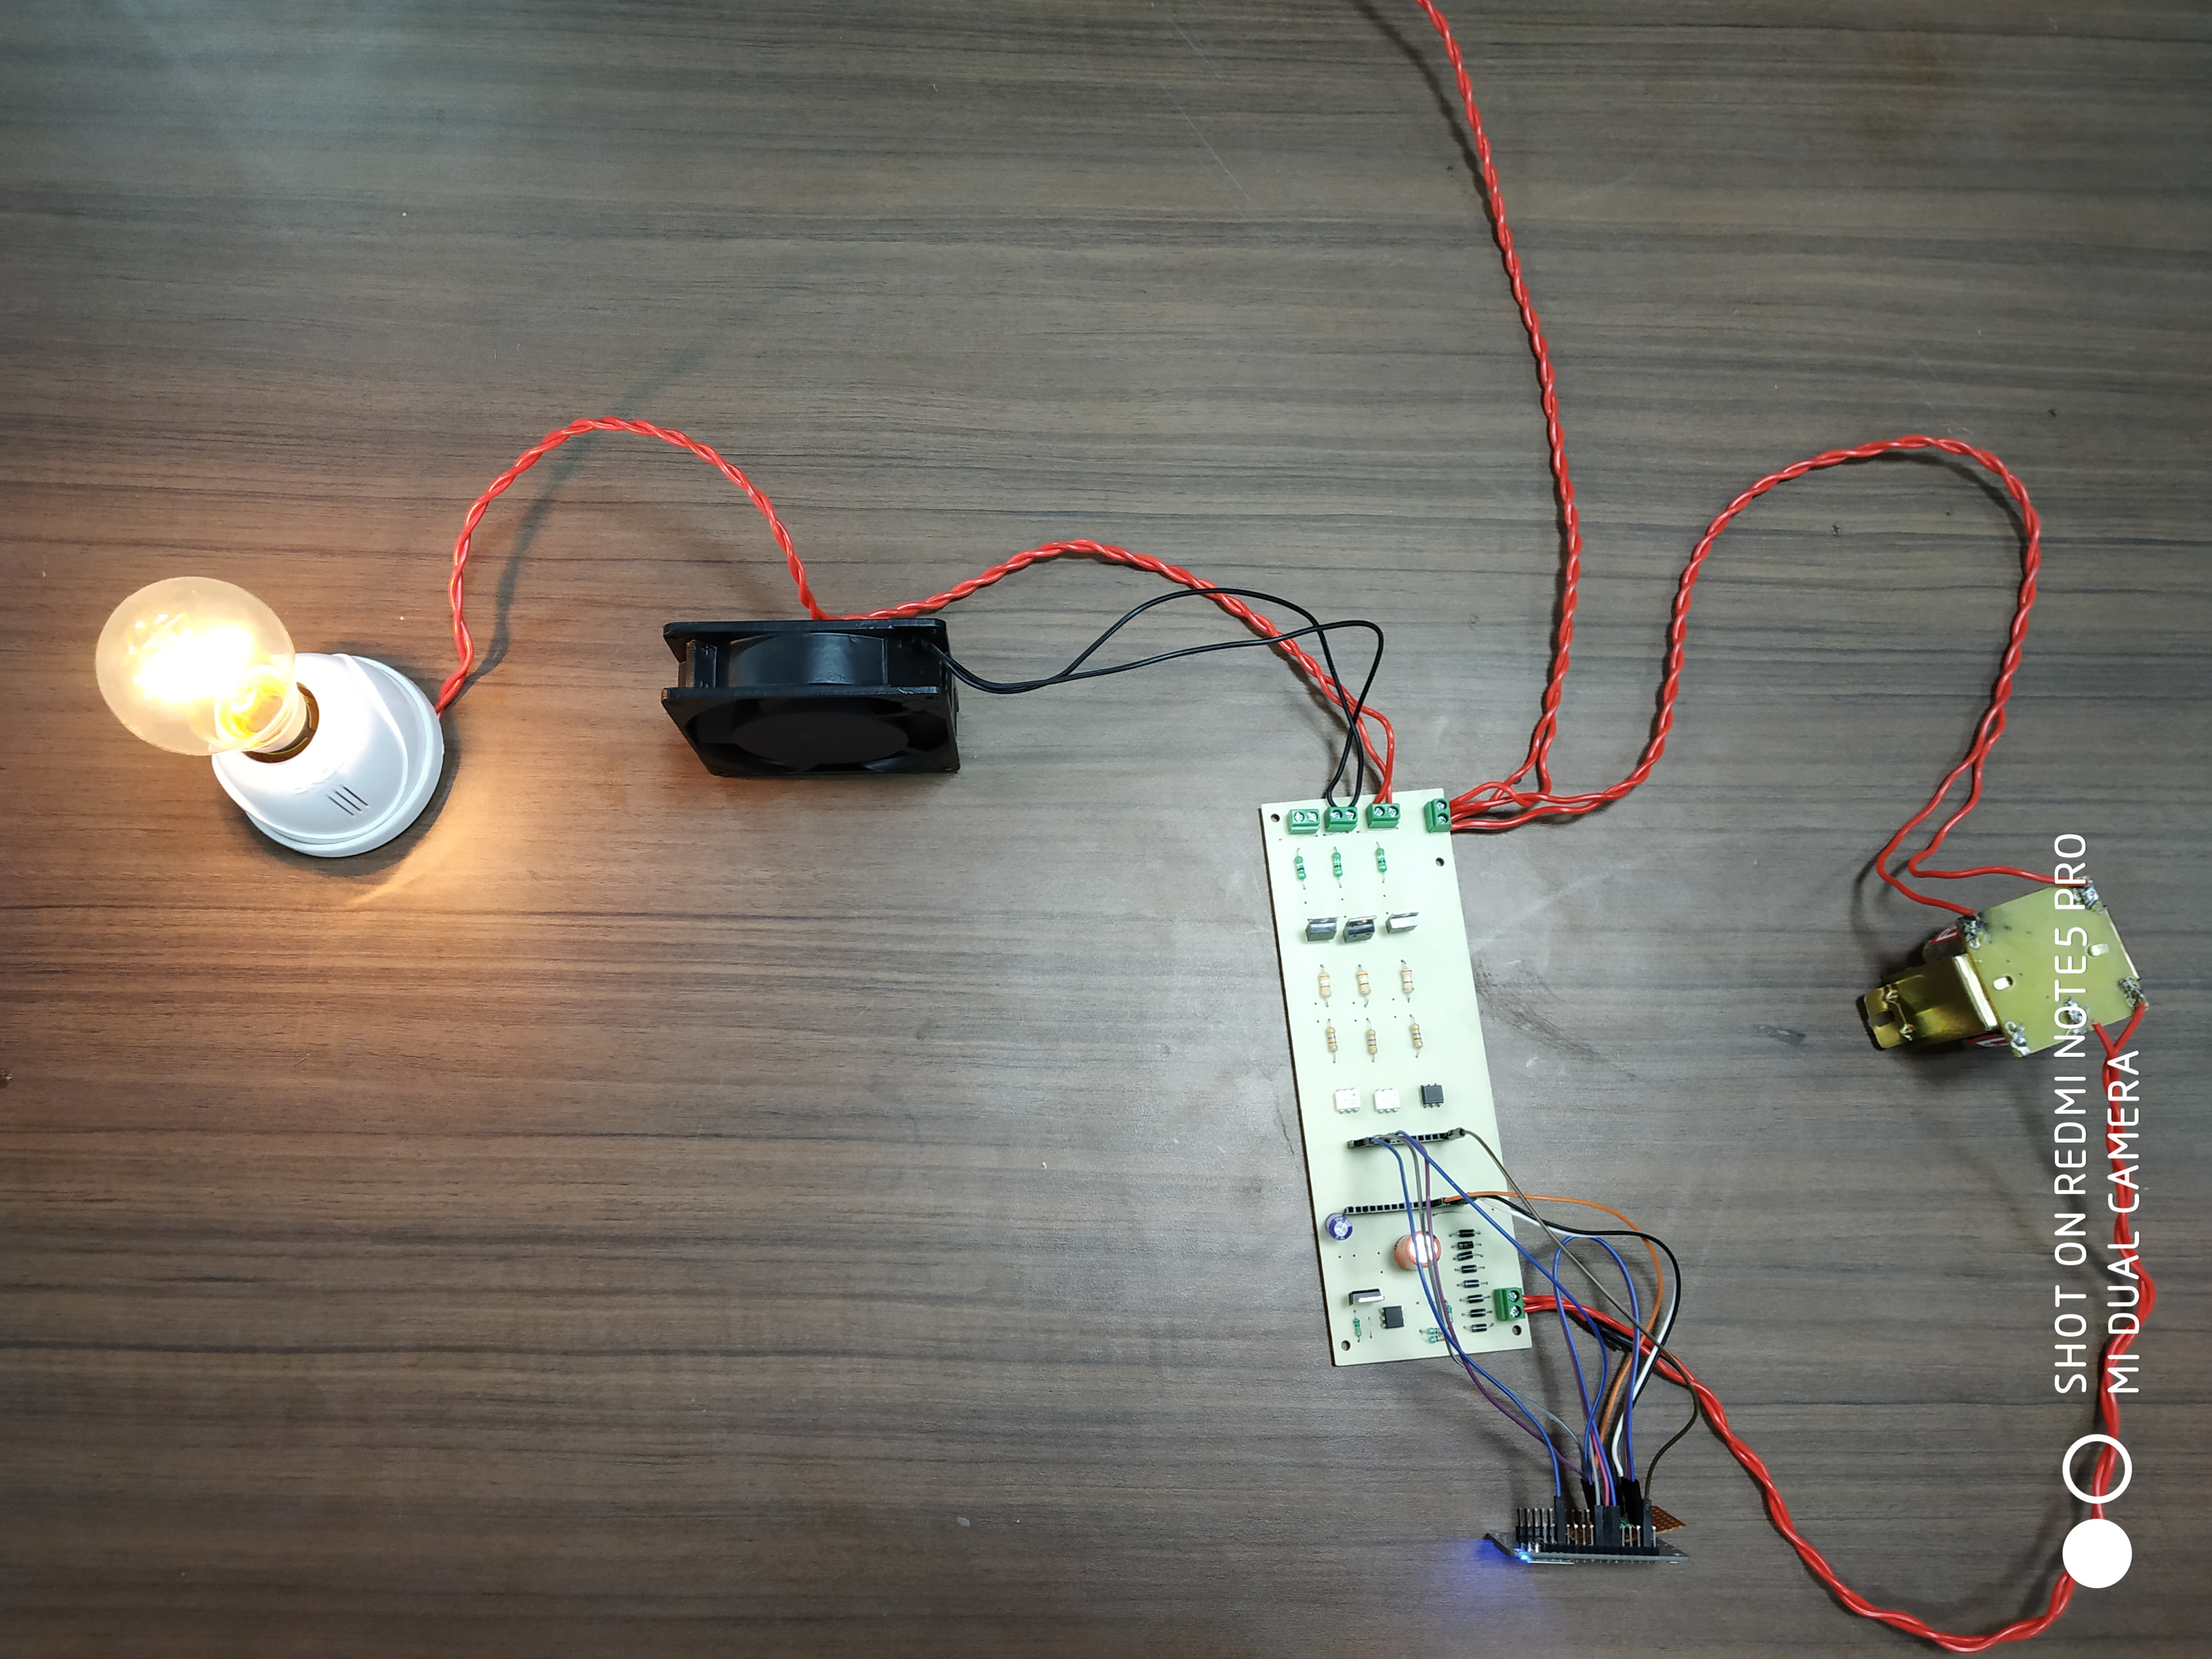
\includegraphics[width=\textwidth]{photos/hardware/Working1.jpg}
	        	\caption{Demonstration of the complete project}
	        \end{figure}

			\begin{figure}[h!]
				\includegraphics[width=\textwidth]{photos/hardware/Working3.jpg}
				\caption{Demonstration of the complete project}
			\end{figure}  
	     \chapter{Results and Discussion}
        \section{Results and Discussion}
        
        \begin{figure}[h!]
        	\centering
        	\includegraphics[width=0.8\textwidth]{photos/results/InterruptTriggerofmicrocontroller.jpg}
        	\caption{Gate signal for the driver circuit}
        \end{figure}
	    \begin{figure}[H]
	    	\centering
	    	\includegraphics[width=0.8\textwidth]{photos/results/ZeroCrossingCircuitWaveform.jpg}
	    	\caption{Shifted Firing pulses lead to reduced apparent voltage}
	    \end{figure}
        \begin{figure}[H]
        	\centering
        	\includegraphics[width=0.8\textwidth]{photos/results/RectifiedOutputVoltage.jpg}
        	\caption{Rectified Output for Zero Detection}
        \end{figure}
    \newpage
        \section{Justification of objectives achieved}
         \begin{enumerate}
	         \item With the help of power electronics devices such as triac, optocoupler etc., we designed the control circuitry for controlling the speed of fan, brightness of lights etc. We have also provided socket (Switch On/Off) for external device connection. A ripple free constant power supply of 5V for power supply of the microcontroller is designed using full bridge rectifier and smoothing capacitors. A zero cross detection circuit is also designed for detection of zero instant of the AC mains so that a reliable firing pulse can be generated from microcontroller in order to control the appliances.
			\item Programming of the microcontroller is done on NodeMCU platform. The coding of the microcontroller is done in C++ language. The program formed allows the microcontroller to generate PWM gating pulses based on the user input to achieve the desired output by the user.
			\item For the user interaction mobile applications enlisting rooms of each household. The rooms are further divided into lists of appliances which provides control over the devices to the user over the internet. The application is made simple and handy for the user to access easily.
         \end{enumerate}
   
	    \chapter{Conclusion and Future Work}
        \section{Conclusion}
        We successfully completed the following work areas, including their simulations and hardware representation:
			\begin{enumerate}
				\item 5V Supply for Microcontroller Power Supply.
				
				\item Zero Crossing Circuit for detection of Zero Voltage instant of AC supply.
				
				\item Firing pulse generation based on Zero Crossing Circuit fed as input to microcontroller.
				
				\item On/Off and dimming control of lamp and fan using Optoisolators and Triac.
				
				\item Android application for managing and control of lamp.
			\end{enumerate}
        \section{Future Work}
        The project can involve further development of-
		\begin{itemize}
			\item Plug and Play modules for AC and other household appliances.
			
			\item Machine Learning based autonomy algorithms.
			
			\item A centralised Home Automation Software to coordinate between various switchboard modules and house the machine learning algorithms.
			
			\item Sensor Aggregator Modules to provide environmental parameters to the device
		\end{itemize}
    
	    \chapter{Project Metrics}
        \section{Challenges faced and Troubleshooting}
        \section{Relevant Subjects}
        	\begin{center}
        		\begin{description}
        			\item [UTA007 Computer Programming-I] 
        			Fundamentals of functional programming
        			\item [UTA009 Computer Programming-II] 
        			Fundamentals of object oriented programming
        			\item [UTA011 Engineering Design-III] 
        			Embedded system design using sensors and micro-controllers
        			\item [UEE301 Direct Current Machines and Transformers]
        			Study of transformers
        			\item [UEE505 Analog and Digital Systems] 
        			Study of analog and digital systems and their interoperability.
        			\item [UEE401 Alternating Current Machines] 
        			Study of the single phase induction motors
        			\item [UEE504 Power Electronics] 
        			Use of switches to control device output in an efficient manner
        			\item [UEI404 Digital Signal Processing Fundamentals] 
        			Use of DSP techniques to process signal from sensors and other devices
        			\item [UEI609 Fundamentals of Microprocessors and Microcontrollers] 
        			% Fundamentals of Assembly Programming and Embedded system design using micro-controllers 
        			\item [UEI501 Control Systems] 
        			Use of closed loop systems to eliminate errors in a system 
        			\item [UEE801 Electric Drives] 
        			Application of Power electronics to control AC Drives
        		\end{description}
        	\end{center}
        \section{Interdisciplinary Aspect}
        	This project consists of extensive multidisciplinary efforts.
        	The Load Optimization algorithm will be generated using a Deep Reinforcement Learning model which is primarily a topic of interest in Computer Science.
        	The wireless communication among the sensors, devices and the HAU are subjects of Electronics and Communication Engineering.\\
        \section{Components Used}
	        \subsection{Software Used}	
	        Provided by college
	        \begin{itemize}
	        	\item MATLAB
	        	\item LabVIEW
	        	\item Multisim and Ultiboard
	        \end{itemize}
	        Open Source
	        \begin{itemize}
	        	\item Tensorflow
	        	\item Node.js
	        \end{itemize}
	        %Hardware to be used: (Details specifications and purpose of each equipment)
	        \subsection{Hardware Used}
	        \begin{itemize}
	        	\item PCB Prototyping Machine
	        	\item Digital Storage Oscilloscope
	        	\item Function Generator
	        	\item Multimeter
	        	\item Soldering station
	        	\item Mobile Phone
	        \end{itemize}
        \section{Brief analytic notes}
        \section{Team Assessment Matrix}
	        \begin{table}[h!]
	        	\begin{tabular}{| l | c | c | c | c |}
	        		\hline
	        		& \multicolumn{4}{c|}{\textbf{Evaluation of}} \\\hline
	        		\textbf{Evaluation by} & Satyam Kumar & Shubham Gupta & Stuti Sidhu & Swanav Swaroop \\
	        		\hline
	        		Satyam Kumar   & 5.0 & 4.5 & 4.5 & 4.5\\
	        		\hline
	        		Shubham Gupta  & 4.5 & 5.0 & 4.5 & 4.5\\
	        		\hline
	        		Stuti Sidhu    & 4.5 & 4.5 & 5.0 & 4.5 \\
	        		\hline
	        		Swanav Swaroop & 4.5 & 4.5 & 4.5 & 5.0 \\ [1ex] 
	        		\hline
	        	\end{tabular}
		        \caption{Team Assessment Matrix}
	        \end{table}
        \section{Work Schedule}
        \begin{table}
        	 {\centering
        		\begin{ganttchart}[expand chart=\textwidth]{1}{12}
        			\gantttitle{2018}{12} \\
        			\gantttitlelist[]{1,...,12}{1} \\
        			\ganttbar{Literature Survey}{4}{4} \\
        			\ganttgroup{WP 1}{4}{6} \\
        			\ganttbar{WP1.1}{4}{4} \\
        			\ganttlinkedbar{WP1.2}{5}{6} \ganttnewline
        			\ganttmilestone{Completion}{6} \ganttnewline
        			\ganttgroup{WP 2}{4}{6} \\
        			\ganttbar{WP2.1}{4}{5} \\
        			\ganttlinkedbar{WP2.2}{5}{6} \ganttnewline
        			\ganttmilestone{Completion}{6} \ganttnewline
        			\ganttgroup{WP 3}{4}{7} \\
        			\ganttbar{WP3.1}{4}{7} \ganttnewline
        			\ganttmilestone{Completion}{7} \ganttnewline
        			\ganttgroup{WP 4}{8}{11} \\
        			\ganttbar{WP4.1}{8}{11} \\
        			\ganttbar{WP4.2}{10}{11} \ganttnewline
        			\ganttmilestone{Completion}{11} \ganttnewline
        			\ganttbar{Integration}{12}{12}
        			\ganttlink{elem2}{elem3}
        			\ganttlink{elem6}{elem7}
        			\ganttlink{elem9}{elem10}
        			\ganttlink{elem12}{elem14}
        			\ganttlink{elem13}{elem14}
        			
        			\ganttlink{elem3}{elem15}
        			\ganttlink{elem7}{elem15}
        			\ganttlink{elem10}{elem15}
        			\ganttlink{elem14}{elem15}
        		\end{ganttchart}
        	}
        \caption{Work Schedule for the complete project}
        \end{table}

        \section{Student Outcome Mapping}
        	\begin{table}[h!]
        		\begin{tabular}{|m{0.75cm}|m{2.75in}|m{2.75in}|}\hline
        		A1.&Applied mathematics (partial differentiation, vector calculus, linear algebra, complex variables, Laplace transform, probability, statistics, discrete mathematics etc.) to obtain analytical, numerical and statistical solutions.&\\\hline
        		A2 & Demonstrate and apply knowledge of fundamentals, scientific and engineering principles towards solving engineering problems.&\\\hline
        		B2 & Utilize suitable hardware equipment for data collection.&\\\hline
        		B3 & Analyze and validate experimental results using appropriate techniques.&\\\hline
        		D1 & Share responsibility and information schedule with others in team.&\\\hline
        		E1 & Classify information to identify engineering problems.&\\\hline
        		E3 & Use analytical, computational and/or experimental methods to obtain solutions.&\\\hline
        		G1 & Prepare and present variety of documents such as project or laboratory reports and inspection reports with discipline specific standards.&\\\hline
        		H1 & Aware of societal and global changes due to engineering innovations.&\\\hline
        		I1 & Able to use resources to adopt new technologies not included in curriculum.&\\\hline
        		J2 & Recognize the impact of engineering decisions reduces on energy resources and environment.&\\\hline
        		K3 & Able to analyze engineering problems using software tools.&\\\hline
        		\end{tabular}
        	\end{table}
    
  
    \backmatter
    	\chapter{References}
\begin{enumerate}
	\item Archana N. Shewale, \textbf{"Renewable Energy Based Home Automation System Using ZigBee"}, International Journal of Computer Technology and Electronics Engineering (IJCTEE), 2015
	
	\item S. Anusha, \textbf{"Home Automation using ATmega328 Microcontroller and Android application"}, International Research Journal of Engineering and Technology(IRJET), 2015
	
	\item J. Chandramohan, \textbf{"Intelligent Smart Home Automation and Security System Using Arduino and Wi-Fi"}, International Journal of Engineering and Computer Science, 2017
	
	\item Kumar Mandula, \textbf{"Mobile based home automation using Internet of Things(IoT)"}, IEEE International Conference, 2015
	
	\item Debraj Basu, \textbf{"Wireless Sensor Network Based Smart Home: Sensor Selection, Deployment and Monitoring"}, IEEE, 2013
	
	\item Byeongkwan Kang, \textbf{"IoT-based monitoring system using tri-level context making model for smart home services"}, IEEE International Conference, 2015
	
	\item Jeya Jeya Padmini, \textbf{"Effective Power Utilization and Conservation in Smart Home Using IoT"}, IEEE International Conference, 2015
	
	\item Pranay P. Gaikwad, \textbf{"A Survey based on Smart Home System Using Internet of Things"}, IEEE International Conference, 2015
\end{enumerate}
    	\chapter{Annexures}
        \section{Code}
        \section{Datasheet of Components}
	        \includepdf[pages={1-2}]{datasheets/bt136}
        	\includepdf[pages={1-2}]{datasheets/4n25}
        	\includepdf[pages={1-2}]{datasheets/moc3021}
        	\includepdf[pages={2-5}]{datasheets/moc3041}
    
    	\addcontentsline{toc}{chapter}{Plagiarism Report}
\includepdf[pages={31-32}]{chapters/backmatter/plagiarism-report}
\end{document}
